% Olympus v2 — iperf3 flow start & oc_bridge -> worker hand-off (abstract)
% bridge_handoff.tex — single-column version: an iperf3 flow starts with its
% client source port pinned to P (--cport=P); oc_bridge waits for a flow on
% port P, duplicates its socket fd, and execl()s into the Python worker --
% same OS process, so the fd (and OC_* env) survive and the worker drives
% the flow's cwnd directly. Full mechanics: bridge_handoff_detailed.tex.
% Compile standalone:  pdflatex bridge_handoff.tex
\documentclass[tikz,border=5pt]{standalone}
\usepackage{tikz}
\usepackage{amssymb}
\usepackage{helvet}
\renewcommand{\familydefault}{\sfdefault}
\usetikzlibrary{arrows.meta,positioning,fit,backgrounds}

\begin{document}
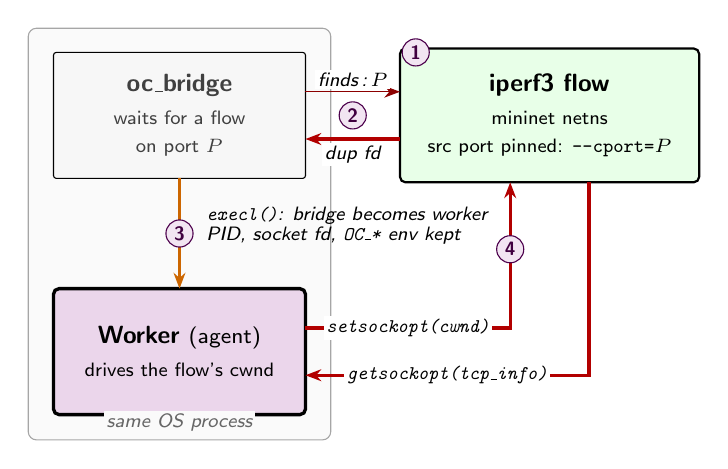
\begin{tikzpicture}[
  font=\small,
  >={Stealth[length=2mm]},
  proc/.style={draw,rounded corners=2pt,thick,minimum height=8mm,
               minimum width=24mm,align=center,fill=blue!7},
  net/.style={draw,rounded corners=2pt,thick,minimum height=8mm,
              minimum width=30mm,align=center,fill=green!9},
  agent/.style={proc,fill=violet!16,very thick},
  bridge/.style={draw,solid,thin,rounded corners=1pt,
                 minimum height=8mm,minimum width=24mm,align=center,
                 fill=black!3,text=black!75},
  band/.style={draw,rounded corners=3pt,thin,draw=black!35,fill=black!2},
  stepnum/.style={circle,draw=violet!60!black,fill=violet!10,inner sep=0.45mm,
                  font=\scriptsize\bfseries,text=violet!50!black},
  data/.style={->,very thick,draw=red!70!black},
  tap/.style={->,thin,draw=red!55!black},
  cfg/.style={->,thick,draw=orange!80!black},
  lbl/.style={font=\scriptsize\itshape,fill=white,inner sep=1pt},
]

% the flow: an iperf3 client whose source port is pinned to P
\node[net,minimum width=38mm,minimum height=17mm] (flow) at (63mm,0mm)
     {\textbf{iperf3 flow}\\[1pt]
      \scriptsize mininet netns\\[-1pt]
      \scriptsize src port pinned: \texttt{-{}-cport=$P$}};
\node[stepnum] at (46mm,8mm) {1};

% the listener
\node[bridge,minimum width=32mm,minimum height=16mm] (bridgebox) at (16mm,0mm)
     {\textbf{oc\_bridge}\\[1pt]
      \scriptsize waits for a flow\\[-1pt]
      \scriptsize on port $P$};

% the worker it turns into
\node[agent,minimum width=32mm,minimum height=16mm] (worker) at (16mm,-30mm)
     {\textbf{Worker} \footnotesize(agent)\\[1pt]
      \scriptsize drives the flow's cwnd};

% both live in the same OS process: exec replaces the image, keeps PID + fd
\begin{scope}[on background layer]
  \node[band,fit=(bridgebox)(worker),inner sep=3mm] (pidband) {};
\end{scope}
\node[font=\scriptsize\itshape,text=black!60,anchor=south,fill=black!2,
      inner sep=1pt] at ([yshift=0.8mm]pidband.south) {same OS process};

% (2) the bridge finds the flow by its pinned port and grabs the socket
\draw[tap]  (32mm,3mm)  -- node[lbl,above=0.3mm]{finds\,:\,$P$} (44mm,3mm);
\draw[data] (44mm,-3mm) -- node[lbl,below=0.3mm]{dup fd}        (32mm,-3mm);
\node[stepnum] at (38mm,0mm) {2};

% (3) exec: the listener becomes the worker
\draw[cfg,very thick] (16mm,-8mm) -- (16mm,-22mm);
\node[stepnum] at (16mm,-15mm) {3};
\node[align=left,anchor=west,font=\scriptsize\itshape,inner sep=1pt]
      at (19mm,-14mm)
      {\texttt{execl()}: bridge becomes worker\\[-1pt]
       PID, socket fd, \texttt{OC\_*} env kept};

% (4) control loop on the inherited socket
\draw[data] (32mm,-27mm)
      -- node[lbl]{\texttt{setsockopt(cwnd)}} (58mm,-27mm)
      -- (58mm,-8.5mm);
\node[stepnum] at (58mm,-17mm) {4};

\draw[data] (68mm,-8.5mm) -- (68mm,-33mm)
      -- node[lbl]{\texttt{getsockopt(tcp\_info)}} (32mm,-33mm);

\end{tikzpicture}
\end{document}
